\documentclass[11pt,twocolumn]{article}
\usepackage[utf8]{inputenc}
\usepackage[spanish]{babel}
\usepackage{amsmath}
\usepackage{hyperref}
\usepackage{graphicx}
\usepackage{fancyhdr}
\usepackage{cite}
\usepackage[left=2cm,top=1cm,right=2cm,nohead]{geometry}
\bibliography{referencias}
\usepackage{cancel}
\usepackage{float}

\title{Acero 304 }
\author{Gustavo Vergara Pareja  \\ Universidad De Córdoba}

\begin{document}

\twocolumn[
\begin{@twocolumnfalse}
\maketitle
\begin{abstract}

En esta practica de laboratorio estudiamos la caída libre, mediante el lanzamiento de una canica a una altura específica, tomar apuntes y entender cómo se comporta este movimiento que presenta aceleración constante con movimiento rectilíneo.
\end{abstract}
\end{@twocolumnfalse}
]
\section{Objetivos}
\begin{itemize}
    \item Determinar la ley distancia-tiempo para la caída libre
    
    \item Determinar la ley velocidad-tiempo para la caída libre
    \item Determinar la aceleración debida a la gravedad
    
\end{itemize}

\section{Marco Teórico}

La caída libre es un movimiento rectilíneo uniformemente acelerado (m.r.u.a.) o movimiento rectilíneo uniformemente variado (m.r.u.v.) en el que se deja caer un cuerpo verticalmente desde cierta altura y no encuentra resistencia alguna en su camino. Las ecuaciones de la caída libre son: \cite{ref_1}.\\

$$y_{f}=y_{1}+v_{1}\cdot t+\frac{1}{2}a\cdot t^{2}$$
$$y_{f}=+v_{1}a\cdot t$$
$$v_{f}^{2}=v_{i}^{2}+2a\Delta y$$

Se deben dejar claras las condiciones que se deben tener en cuenta para que un movimiento se considere caída libre, estas condiciones se conocen como las leyes fundamentales de la caída libre y son:\cite{ref_2}\\

\begin{itemize}

\item Todos los cuerpos que tengan una caída libre tienen una trayectoria estrictamente vertical, no hay desviación en el recorrido de ningún tipo.

\item La caída libre de los cuerpos es un caso del movimiento uniformemente acelerado.

\item Todos los cuerpos caen con la misma aceleración si se dejan caer en el mismo lugar porque la única influencia es la gravedad.

\item Todos los cuerpos que se dejan caer en el vacío se demoran el mismo tiempo en alcanzar la misma velocidad.

\end{itemize}

\begin{figure}[h]
    \centering
    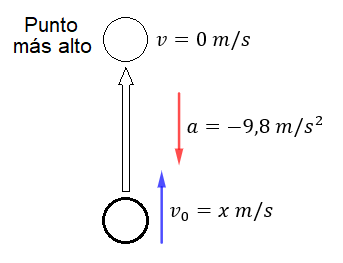
\includegraphics[width=7 cm, height=5cm]{ImagenI.png}
    \caption{Caída Libre}
    \label{fig:my_label}
\end{figure}


\section{Materiales}
Disparador de balín\\
Contador de milisegundos\\
Regla 1000mm\\
Soporte\\
Cables conectores\\
Platillo interruptor\\

\section{Montaje y Procedimiento}

\begin{figure}[h]
    \centering
    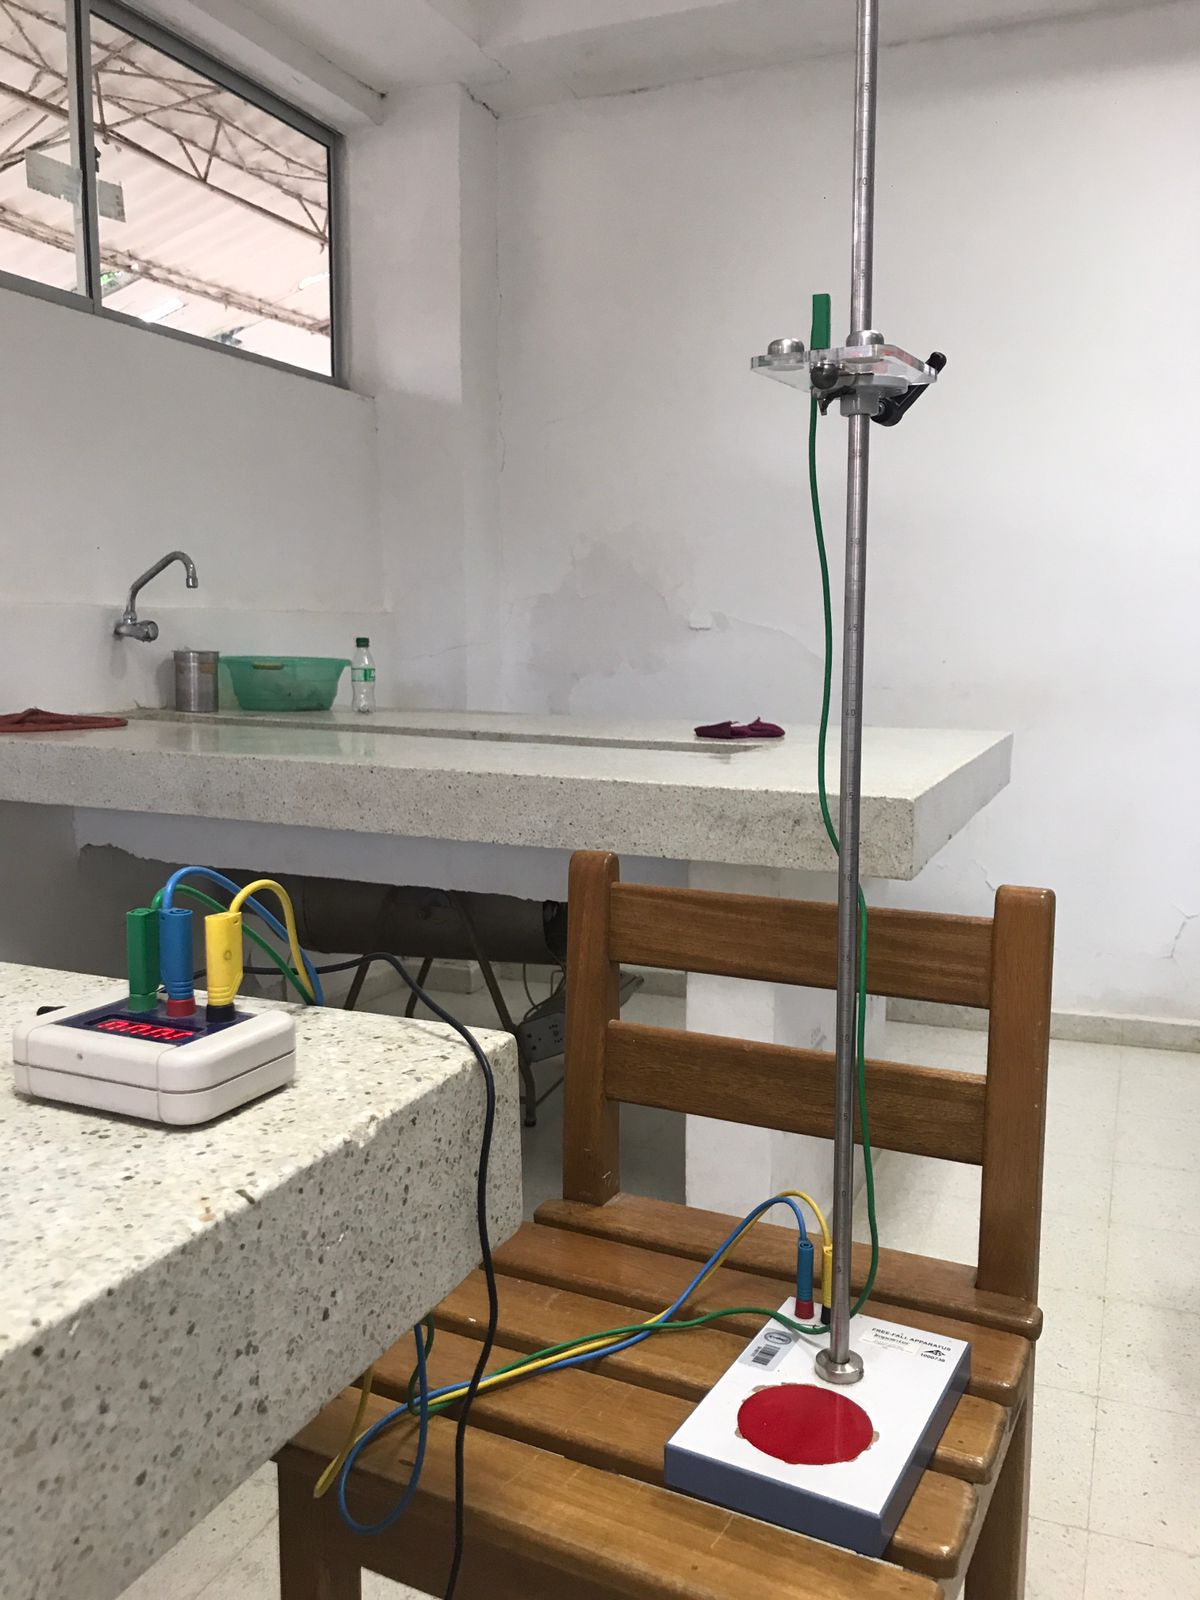
\includegraphics[width=7 cm, height=5cm]{Imagen II.jpeg}
    \caption{Montaje}
    \label{fig:my_label}
\end{figure}

Se tomó un balín el cual era colocado en en la cima de un soporte. El balín se dejaba caer desde diferentes alturas, repitiendo el procedimiento varias veces en una misma alturas. Al caer, había un censor que registraba el tiempo en caer del balín, tomamos los datos correspondientes. 

\section{Evaluación}

\begin{enumerate}
    \item ¿Depende el tiempo de caída de un cuerpo de su peso? Explique su respuesta.

    \item Realice la gráfica de altura (h) en función del tiempo (t). ¿Qué tipo de gráfica obtiene?

    \item ¿Qué relación existe entre la distancia recorrida y el tiempo?

    \item Trace varias rectas tangentes a la gráfica $h$ vs $t$ en distintos puntos. ¿Qué unidades tienen las pendientes de esas rectas?¿Qué significado físico poseen?¿Tienen el mismo valor en todos los puntos?¿Esperaba esta respuesta?

    \item Realice la gráfica de altura (h) en función del tiempo al cuadrado $\left(t^{2}\right)$ ¿Qué tipo de gráfica obtiene?

    \item Halle la pendiente de la gráfica de altura (h) en función del tiempo al cuadrado $\left(t^{2}\right)$ ¿Qué unidades posee?

    \item Halle la ecuación que relaciona las variables $h$ y $t$.

    \item ¿Qué posibles errores se cometieron en la realización del experimento y cómo los corregiría?

    \item ¿Es posible determinar el valor de la aceleración de la gravedad usando los datos del anterior experimento? Si su respuesta es afirmativa calcúlela, en caso contrario, justifique.

    \item ¿Conoce situaciones reales en las cuales se presente este tipo de movimiento en la naturaleza?

\end{enumerate}


\section{Respuestas}

\begin{enumerate}

\item \textbf{¿Depende el tiempo de caída de un cuerpo de su peso? Explique su respuesta.}\\

No, ya que si tenemos un sistema en el cual despreciamos la resistencia del aire y dejamos caer dos objetos de diferente peso, estos caerán en el mismo intervalo de tiempo, ya que todos los cuerpos en la tierra experimentan una fuerza de atracción o aceleración constante que es la gravedad.\\
    

\item  \textbf{Realice la gráfica de altura (h) en función del tiempo (t). ¿Qué tipo de gráfica obtiene?}\\

\begin{figure}[H]
    \centering
    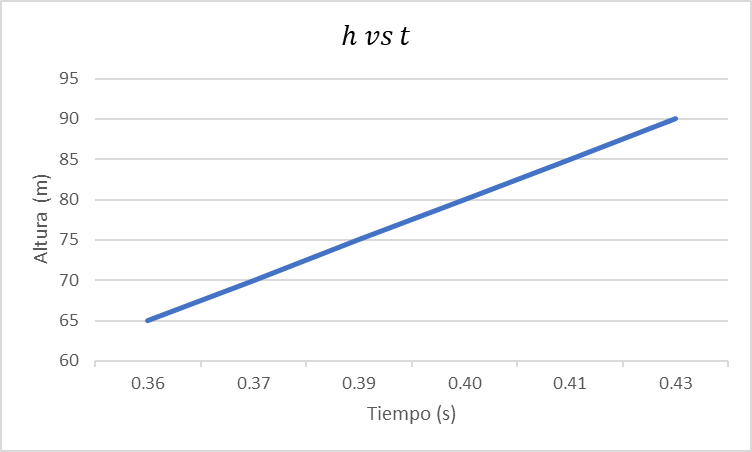
\includegraphics[width=7 cm,height=5cm]{Imagen5.png}
    \caption{$h$ vs $t$}
    \label{fig:my_label}
\end{figure}


\item \textbf{¿Qué relación existe entre la distancia recorrida y el tiempo?}.\\

La relación que existe entre la distancia recorrida y el tiempo es directamente proporcional a la raíz que aumentan la distancia en la misma forma que lo hace el tiempo.\\


 \item \textbf{Trace varias rectas tangentes a la gráfica $h$ vs $t$ en distintos puntos. ¿Qué unidades tienen las pendientes de esas rectas?¿Qué significado físico poseen?¿Tienen el mismo valor en todos los puntos?¿Esperaba esta respuesta?}\\
 
$$m_{1}=\frac{70cm-65cm}{0.37s-0.36s}=500 cm/s\rightarrow 0.5m/s$$

$$m_{2}=\frac{75cm-70cm}{0.393s-0.379s}=357.1cm/s\rightarrow 0.357m/s$$

$$m_{3}=\frac{80cm-75cm}{0.405s-0.343s}=416cm/s\rightarrow 0.416m/s\\
$$

$$m_{4}=\frac{85cm-80cm}{0.418s-0.405s}=384.6cm/s\rightarrow 0.38m/s$$

\begin{itemize}
    \item ¿Qué unidades tienen las pendientes de esas rectas?\\

    Están expresadas en $m/s$\\

    \item \textbf{¿Qué significado físico poseen?}\\

    Esta representa la velocidad y esta dada en diferentes intervalos de tiempos.\\

    \item \textbf{¿Tienen el mismo valor en todos los puntos?¿Esperaba esta respuesta?}\\

    No, debido a que la altura provvoca un cmabio en la velocidad.\\

    \item \textbf{¿Esperaba esta respuesta?}\\

    Se esperaba que a mayor altura, mayor fuera la velocidad pero esto no siempre se cumple.

    
\end{itemize}

\item \textbf{Realice la gráfica de altura (h) en función del tiempo al cuadrado $\left(t^{2}\right)$ ¿Qué tipo de gráfica obtiene?}\\

\begin{figure}[H]
    \centering
    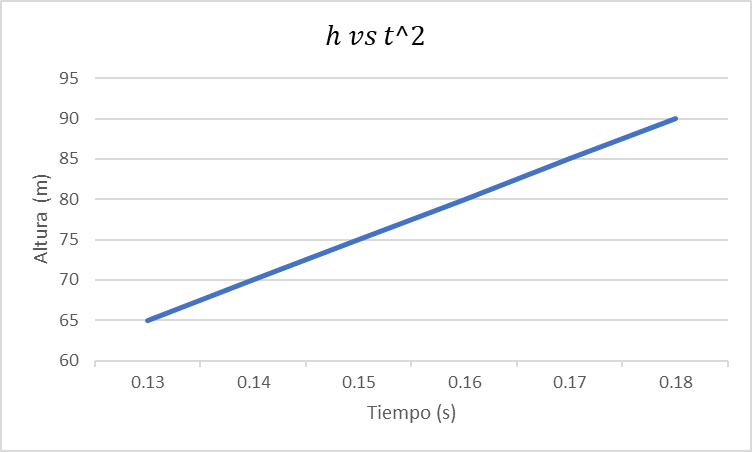
\includegraphics[width=7 cm, height=5cm]{Imagen4.png}
    \caption{Gráfico $h$ vs $t^{2}$}
    \label{fig:my_label}
\end{figure}


\begin{itemize}
    \item \textbf{¿Qué tipo de gráfica obtiene?}

    Y se obtiene una gráfica de líneas

\end{itemize}

 \item \textbf{Halle la pendiente de la gráfica de altura (h) en función del tiempo al cuadrado $\left(t^{2}\right)$ ¿Qué unidades posee?}

 $$m_{1}=\frac{70cm-65cm}{0.14s-0.13s}=500cm/s\rightarrow 0.5m/s$$

 $$m_{2}=\frac{75cm-70cm}{0.154s-0.14s}=357.1cm/s\rightarrow 0.357m/s$$

 $$m_{3}=\frac{80cm-75cm}{0.164s-0.154s}=500cm/s\rightarrow 0.5m/s$$

 $$m_{4}=\frac{85cm-80cm}{0.174s-0.164s}=500cm/s\rightarrow 0.5m/s$$

 $$m_{5}=\frac{90cm-85cm}{0.185s-0.174s}=454.5cm/s\rightarrow 0.45m/s$$
\begin{itemize}
    \item \textbf{¿Qué unidades posee?}\\

    $m/s$
    
\end{itemize}
 

 \item \textbf{Halle la ecuación que relaciona las variables $h$ y $t$.}
    \begin{gather*} 
\frac{h_{f}-h_{i}}{T_{f}-T_{i}}
\end{gather*}
    

\item \textbf{¿Qué posibles errores se cometieron en la realización del experimento y cómo los corregiría?}\\

Posteriormente al tener el mismo histograma elaborado, se calculara el error aleatorio, el error de escala y el error sistematico de una serie de mediciones del experimento de la caida libre del balin hechas en condiciones.

Al momento de caer el cuerpo caia y se quedaba estable y asi altera el resultado del analisis y para corregirla se repetia de nuevo el experimento.



\item \textbf{¿Es posible determinar el valor de la aceleración de la gravedad usando los datos del anterior experimento? Si su respuesta es afirmativa calcúlela, en caso contrario, justifique.}\\

Seria muy dificil obtener el resultado de la gravedad con los datos, pero de ser posible se haria mediante la siguiente formula.

$$g=\frac{2h}{t^{2}}$$


\item \textbf{¿Conoce situaciones reales en las cuales se presente este tipo de movimiento en la naturaleza?}

\begin{itemize}
    \item Arrojar una piedra en un pozo, aplicando fuerza con el brazo para que llegue más rápido.

    \item Una flecha disparada hacia arriba 

    \item Una pelota lanzada hacia arriba 

    \
\end{itemize}
 
\end{enumerate}

\section{Conclusión}

\begin{itemize}
    \item Se determinó la ley distancia-tiempo para la caída libre
    \item Se determinó la ley velocida-tiempo para la caída libre
    \item Se determinó la aceleración debida a la gravedad
\end{itemize}


\section{Bibliografía}
\begin{thebibliography}{}
\bibitem{ref_1}
(Fernández, s/f)
Fernández, J. L. (s/f). Caída Libre. Fisicalab.com. Recuperado el 25 de mayo de 2023, de https://www.fisicalab.com/apartado/caida-libre

\bibitem{ref_2}
(Sanchez, 2021)
Sanchez, L. (2021). Caida Libre. Independently Published.




\clearpage 

\section{Anexos}



\end{thebibliography}{}
\end{document}